% EBP course: session 8
% Several new slides added to this lecture
% Thomas Klee
% 20 Mar 2019

% Preamble
\documentclass{beamer}
\usetheme{Singapore}
\usefonttheme[onlysmall]{structurebold}
\setbeamerfont{title}{shape=\itshape,family=\rmfamily}
\usepackage{graphicx}
\usepackage[english]{babel}
\usepackage[utf8x]{inputenc}
\usepackage{amsfonts, amsmath, amsthm, amssymb} % for math fonts, symbols and environments
\usepackage{xcolor}
\usepackage{booktabs}
\usepackage{ctable} % for command-driven tables
\usepackage{wasysym} 
%\hypersetup{colorlinks, allcolors = ., urlcolor = blue,} % to change color of URL from black to blue
\usepackage[natbibapa]{apacite}
\beamertemplatenavigationsymbolsempty % uncomment to add slide navigation symbols to each slide
\usepackage{appendixnumberbeamer}  % to suppress page numbers on extra slides
\setbeamertemplate{footline}[frame number] % to add slide numbers

% activate following line for custom appearance
% \usepackage{beamerthemesplit} 

\mode<presentation>

% information for title slide
\title{Diagnostic (Classification) Accuracy Studies, part 1}
\subtitle{}
\author{Evidence-Based Practice in Speech-Language Therapy \\ (SHSC 2033)}
\institute{Session 8}
\date{Thomas Klee \& Elizabeth Barrett}
\titlegraphic{
\includegraphics[width=6cm]{images/logo_CE_C.jpg}} % HKU logo

\begin{document}

% create title slide with information above
\begin{frame}
	\titlepage
\end{frame}

% 1
\begin{frame}{Outline}
	\begin{enumerate}
	\item Diagnostic accuracy of clinical tests and measures
	\item Classification accuracy measures
	\item Group discussion
	\end {enumerate}
\end{frame}

\section{Introduction}

% 2
\begin{frame}{Why do we  assess clients?}
	\begin{enumerate}
	\item To detect or rule out a condition (classify)
		\begin{itemize}
		\item[-] Screening
		\item[-] Diagnosis
		\item[-] Differential diagnosis
		\end{itemize}
	\item To track the clinical course of a condition
	\item To measure intervention outcome (or progress)
	\end{enumerate}
\end{frame}

% 3
\begin{frame}{A framework for diagnostic research\footnote{\tiny{\citet{Sackett2002a}}}}
	\begin{block}{Phase I}
		\begin{itemize}
		\item[-]  Do those with the target disorder have different test results than those without the disorder?
		\item[-]  Results at the group level
		\end{itemize}
	\end{block}
	
	\begin{block}{Phase II}
		\begin{itemize}
		\item[-] Are those with certain test results more likely to have the target disorder than those with other test results? \\
		\item[-] Results at the individual level
		\end{itemize}
	\end{block}
\end{frame}

% 4
\begin{frame}{A framework for diagnostic research\footnote{\tiny{\citet{Sackett2002a}}}}
	\begin{block}{Phase III}
		\begin{itemize}
		\item[-]  Does the test distinguish those with and without the target disorder among those in whom it is clinically reasonable to suspect that the disorder is present?
		\item[-]  Results at the individual level
		\end{itemize}
	\end{block}
	
	\begin{block}{Phase IV}
		\begin{itemize}
		\item[-] Do those who undergo the diagnostic test fare better (in their ultimate health outcomes) than similar people who are not tested?
		\end{itemize}
	\end{block}
\end{frame}

% 5
\begin{frame}{Diagnostic quartet\footnote{\tiny{\citet[p. 275]{Haynes2006}}}}
	\begin{block}{A valid diagnostic study\dots}
		\begin{enumerate}
		\item Assembles an appropriate spectrum of patients
		\item Applies both the \textbf{diagnostic test} ("index measure") and the \textbf{reference standard} to all of them
		\item Interprets each blind to the other
		\item Repeats itself in a second, independent (``test") set of patients (replication)
		\end{enumerate}
	\end{block}
\end{frame}

% 6
\begin{frame}{Diagnostic accuracy studies compare\dots}
	\begin{block}{Index measure}
		\begin{itemize}
		\item[-]  The test or measure under investigation
		\end{itemize}
	\end{block}
	
	\begin{block}{Reference standard}
		\begin{itemize}
		\item[-] The way in which the target condition is defined
		\item[-] \alert{Gold standard} is a term used when there is widespread agreement on how the reference standard for a condition should be defined (i.e., a definitive diagnosis).
		\end{itemize}
	\end{block}
\end{frame}

% 7
\begin{frame}{2 x 2 outcome table}
\begin{center}
\begin{tabular}{l | c | c }
\toprule
& Condition & Condition \\
& present & absent \\ 
\hline
Index test $+$ & \alert{True positive} & False positive \\
\hline
Index test $-$ & False negative & \alert{True negative} \\
\bottomrule
\end{tabular}
\end{center}
\end{frame}

% 8
\begin{frame}{2 x 2 outcome table}
\begin{center}
\begin{tabular}{l | c | c }
\toprule
& Condition & Condition \\
& present & absent \\ 
\hline
Index test $+$ & a & b \\
\hline
Index test $-$ & c & d \\
\bottomrule
\end{tabular}
\end{center}
\end{frame}

% 9
\begin{frame}{Example: early identification of language delay}
	\begin{itemize}
	\item[O] How accurate is \footnote{\tiny{Outcome measure is classification accuracy}}
	\item[I]  parent-based screening \footnote{\tiny{Index measure}}
	\item[P] for identifying toddlers in need of further evaluation for suspected language delay
	\item[C] compared to the results of a clinical evaluation? 
	\end{itemize}
\end{frame}

% 10
\begin{frame}{Study details\footnote{\tiny{\citet{Klee2000a, Klee1998}}}}
	\begin{itemize}
	\item 24-month-olds were screened using two questionnaires sent to their parents ($N = 306$).
		\begin{itemize}
		\item[-] Language Development Scale (Rescorla, 1998)
		\item[-] Written questionnaire asking about concerns and other things. 
		\end{itemize}
	\item Double-blind clinical evaluations were done within 1 month of the screening ($N = 64$).
	\item Concurrent and predictive validity of the screening approach were examined. 
	\end{itemize}
\end{frame}

% 11
\begin{frame}{Study measures}
	\begin{block}{Index test}
	[$<50$ words OR no word combinations by 24 months on the LDS]\\
	AND 
	[either parent concern OR $>6$ ear infections]
	\end{block}
	
	\begin{block}{Reference standard}
	Clinical outcome (language delay, language normal) based on standardised test, play-based language sample and clinical judgement. 
	\end{block}
\end{frame}

% 12
\begin{frame}{Screening outcomes\footnote{\tiny{\citet{Klee2000a, Klee2008a}}}}
\begin{center}
\begin{tabular}{l | c | c | c}
\toprule
& Language & Language & \\
& delay & normal & Total \\ 
\hline
Screen $+$ & 10 & 2 & 12 \\
\hline
Screen $-$ & 1 & 51 & 52 \\
\hline
Total & 11 & 53 & 64 \\
\bottomrule
\end{tabular}
\end{center}
\end{frame}

\section{Accuracy Measures}

\begin{frame}
\begin{center}
\Huge{Classification Accuracy Measures}
\end{center}
\end{frame}

% 13
\begin{frame}{Sensitivity}
How accurately does the screen identify those \alert{with} the condition? \\

\begin{center}
\begin{tabular}{l | c | c | c}
\toprule
& Language & Language & \\
& delay & normal & Total \\ 
\hline
Screen $+$ & \alert{10} & 2 & 12 \\
\hline
Screen $-$ & \alert{1} & 51 & 52 \\
\hline
Total & \alert{11} & 53 & 64 \\
\bottomrule
\end{tabular}
\end{center}

\begin{center}
\textbf{Sensitivity}: 10/11 = .91, 95\% CI [.62, 1.00]
\end{center}
\end{frame}

% 14
\begin{frame}{Specificity}
How accurately does the screen identify those \alert{without} the condition? \\

\begin{center}
\begin{tabular}{l | c | c | c}
\toprule
& Language & Language & \\
& delay & normal & Total \\ 
\hline
Screen $+$ & 10 & \alert{2} & 12 \\
\hline
Screen $-$ & 1 & \alert{51} & 52 \\
\hline
Total & 11 & \alert{53} & 64 \\
\bottomrule
\end{tabular}
\end{center}

\begin{center}
\textbf{Specificity}: 51/53 = .96, 95\% CI [.87, .99]
\end{center}
\end{frame}

% 15
\begin{frame}{Positive predictive value}
\begin{center}
What proportion of positive tests are true positives? \\
\end{center}

\begin{center}
\begin{tabular}{l | c | c | c}
\toprule
& Language & Language & \\
& delay & normal & Total \\ 
\hline
Screen $+$ & \alert{10} & \alert{2} & \alert{12} \\
\hline
Screen $-$ & 1 & 51 & 52 \\
\hline
Total & 11 & 53 & 64 \\
\bottomrule
\end{tabular}
\end{center}

\begin{center}
\textbf{PPV}: 10/12 = .83, 95\% CI [.55, .95]
\end{center}
\end{frame}

% 16
\begin{frame}{Negative predictive value}
\begin{center}
What proportion of negative tests are true negatives? \\
\end{center}

\begin{center}
\begin{tabular}{l | c | c | c}
\toprule
& Language & Language & \\
& delay & normal & Total \\ 
\hline
Screen $+$ & 10 & 2 & 12 \\
\hline
Screen $-$ & \alert{1} & \alert{51} & \alert{52} \\
\hline
Total & 11 & 53 & 64 \\
\bottomrule
\end{tabular}
\end{center}

\begin{center}
\textbf{NPV}: 51/52 = .98, 95\% CI [.90, 1.00]
\end{center}
\end{frame}

% 17
\begin{frame}{Caveats}
	\begin{itemize}
	\item All four measures are calculated from a \alert{sample} of data. But what is important to clinicians is how the new test (or screening measure) will perform in the \alert{population}. 
	\item Although sensitivity and specificity values should reflect their population values, PPV and NPV will not, since they vary with \alert{prevalance}.
	\end{itemize}
\end{frame}

% 18
\begin{frame}{Likelihood ratios}
	\begin{itemize}
	\item Indicate how many times more likely particular test results occur in those with the condition than in those without the condition.
	\item Can be directly applied to give probabilistic statements concerning the likelihood of the condition in an individual.
	\end{itemize}
\end{frame}

% 19
\begin{frame}{Positive likelihood ratio (LR+)}
	\begin{itemize}
	\item Likelihood ratio of a positive test result
	\item Indicates the number of times a positive test is likely to occur in those with the disorder compared to those without
	\item Proportion of positive screens in children with language delay / Proportion of positive screens in those without language delay 
	\item LR+ $= Sensitivity / (1 - Specificity)$
	\item LR+ $= .91 / (1 - .96) = 24.1$, 95\% CI [6.1, 95.0]
	\item When a child screens positive, he/she is 24 times more likely to have delayed language than not.
	\item The further LR+ is from 1, the more accurate the classification (diagnostic) ability of the test.
	\end{itemize}
\end{frame}

% 20
\begin{frame}{Negative likelihood ratio (LR--)}
	\begin{itemize}
	\item Likelihood ratio of a negative test result
	\item Indicates the number of times a negative test is likely to occur in those with the disorder compared to those without
	\item Proportion of negative screens in children with language delay / Proportion of negative screens in those without language delay 
	\item LR-- $= (1 - Sensitivity) /  Specificity$
	\item LR-- $= (1 - .91) / .96 = .09$, 95\% CI [.02, .61]
	\item When a child screens negative, he/she is .09 times as likely to have delayed language as not.
	\item The further LR-- is from 1, the more accurate the classification (diagnostic) ability of the test.
	\end{itemize}
\end{frame}

% 21
\begin{frame}{Interpreting LRs\footnote{\tiny{\citet[p. 208]{Guyatt2008d}}}}
	\begin{itemize}
	\item LRs of  $>10$ or $<0.1$ indicate large and often conclusive changes from pre- to post-test probability.
	\item LRs of 5 to 10 and 0.1 to 0.2 indicate moderate shifts in probability.
	\item LRs of  2 to 5 and 0.2 to 0.5 indicate small (but sometimes important) shifts in probability.
	\item LRs of 1 to 2 and 0.5 to 1 alter probability to a small (and rarely important) degree.
	\end{itemize}
\end{frame}

% 22
\begin{frame}{Here's the cool part.}
	\begin{itemize}
	\item You can convert LRs to post-test probabilities. (woop, woop)
	\item Tells you the \textbf{probability} that your client has the disorder, given your test result.
	\item In screening, a large post-test probability would indicate the need for further, clinical assessment (e.g., language sample, informal or formal assessment).
	\end{itemize}
\end{frame}

% 23
\begin{frame}{Converting LRs to post-test probabilities}
	\begin{itemize}
	\item Why? Probabilities are easier to interpret than odds,\footnote{\dots to me anyway!} being on a scale of 0-100.
	\item Post-test probabilities indicate the chance of having the condition given a positive or negative test result.
	\item Post-test probabilities can be calculated from various pre-test probabilities (prevalence figures).
	\item More information about this will be presented next session.
	\end{itemize}
\end{frame}

% -----------------------------------------------------------------------------------
% Slides 24, 25, 26 are in next week's lecture, so not needed here.
% They could be left in if ever needed in a single lecture
% but might want to add a few slides from session 9 
% that are not in session 8 in single lecture is needed.
% -----------------------------------------------------------------------------------

% 24
%\begin{frame}{LR Nomogram\footnote{\tiny{\citet[p. 285]{Haynes2006}}}}
%	\begin{center}
%	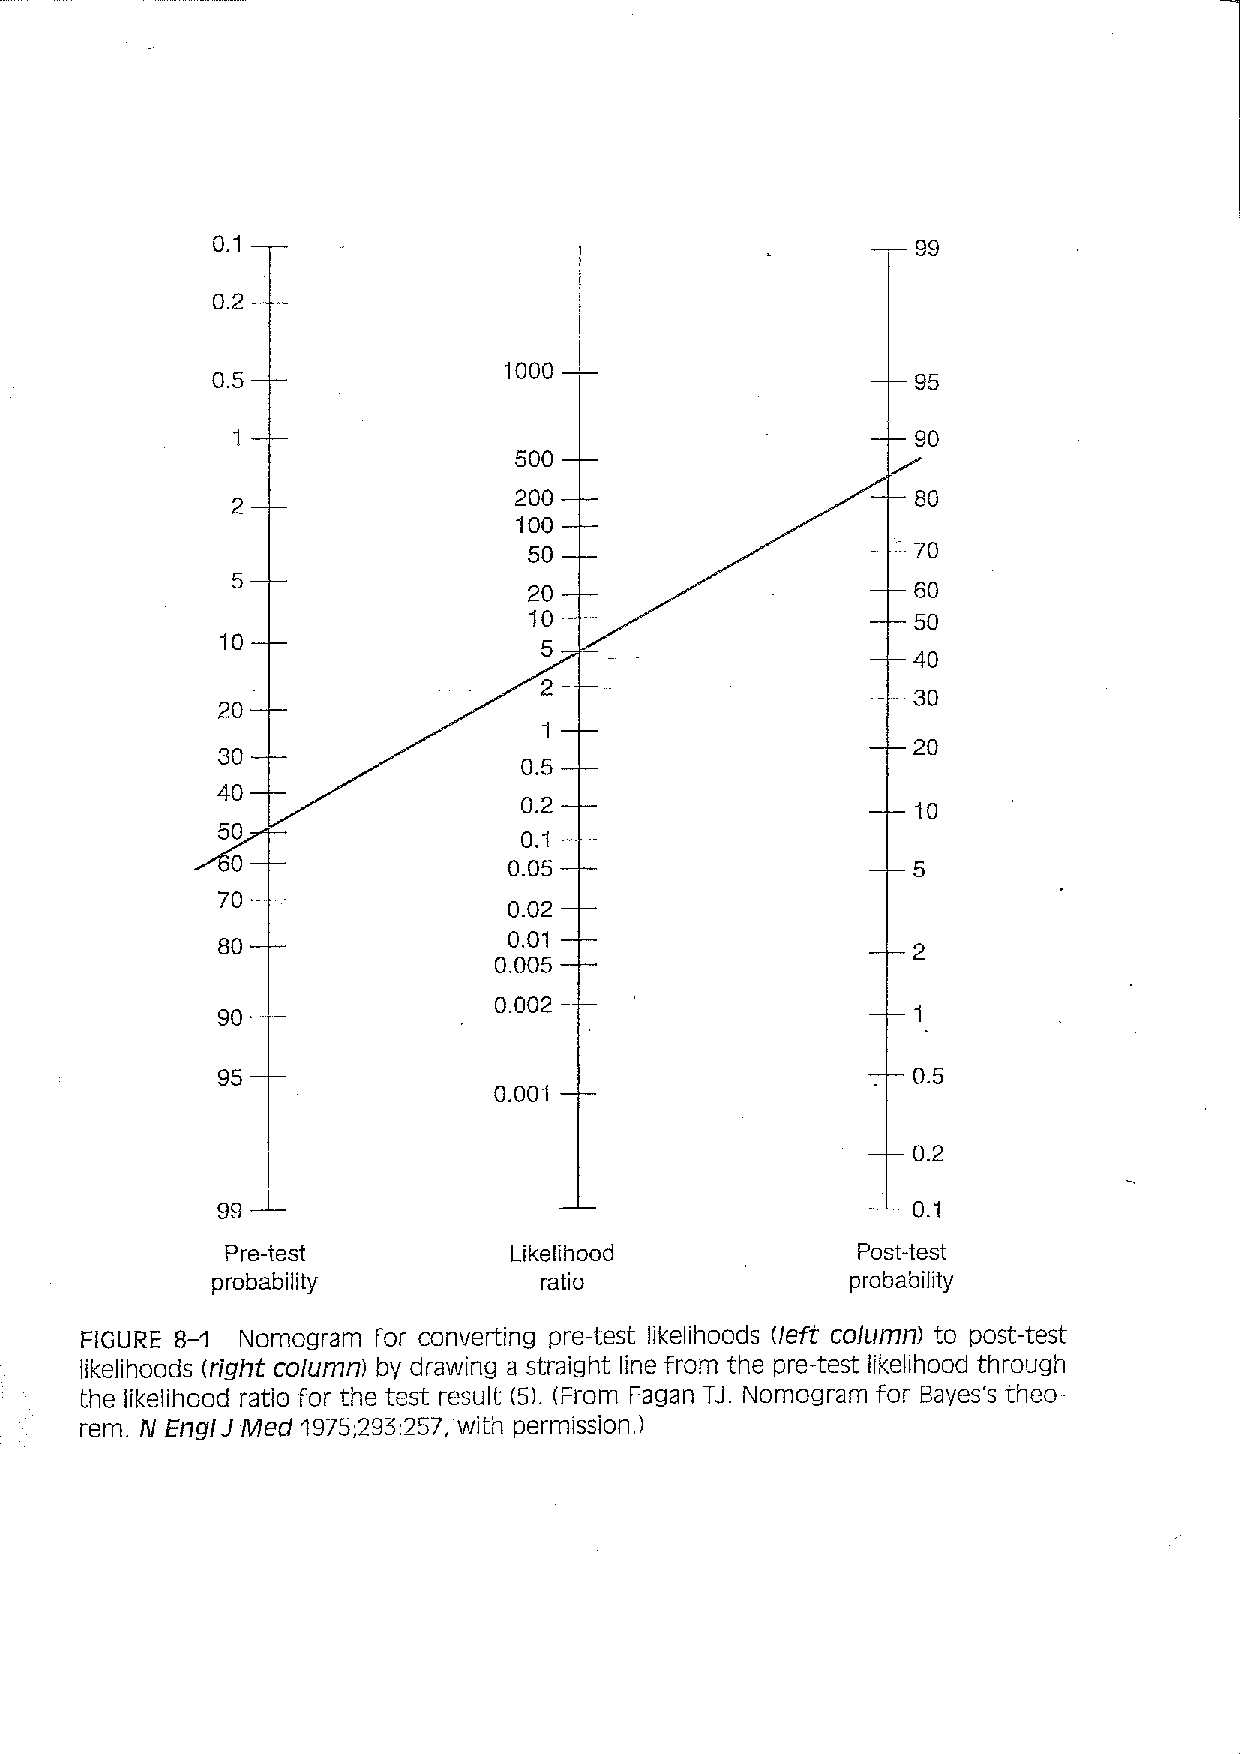
\includegraphics[height=7.5cm]{images/nomogram_haynes_2006.pdf}
%	\end{center}	
%\end{frame}

% 25
%\begin{frame}{Classification metrics using R\footnote{\tiny{\citet{RCoreTeam2016, Stevenson2016}}}}
%	\begin{center}
%	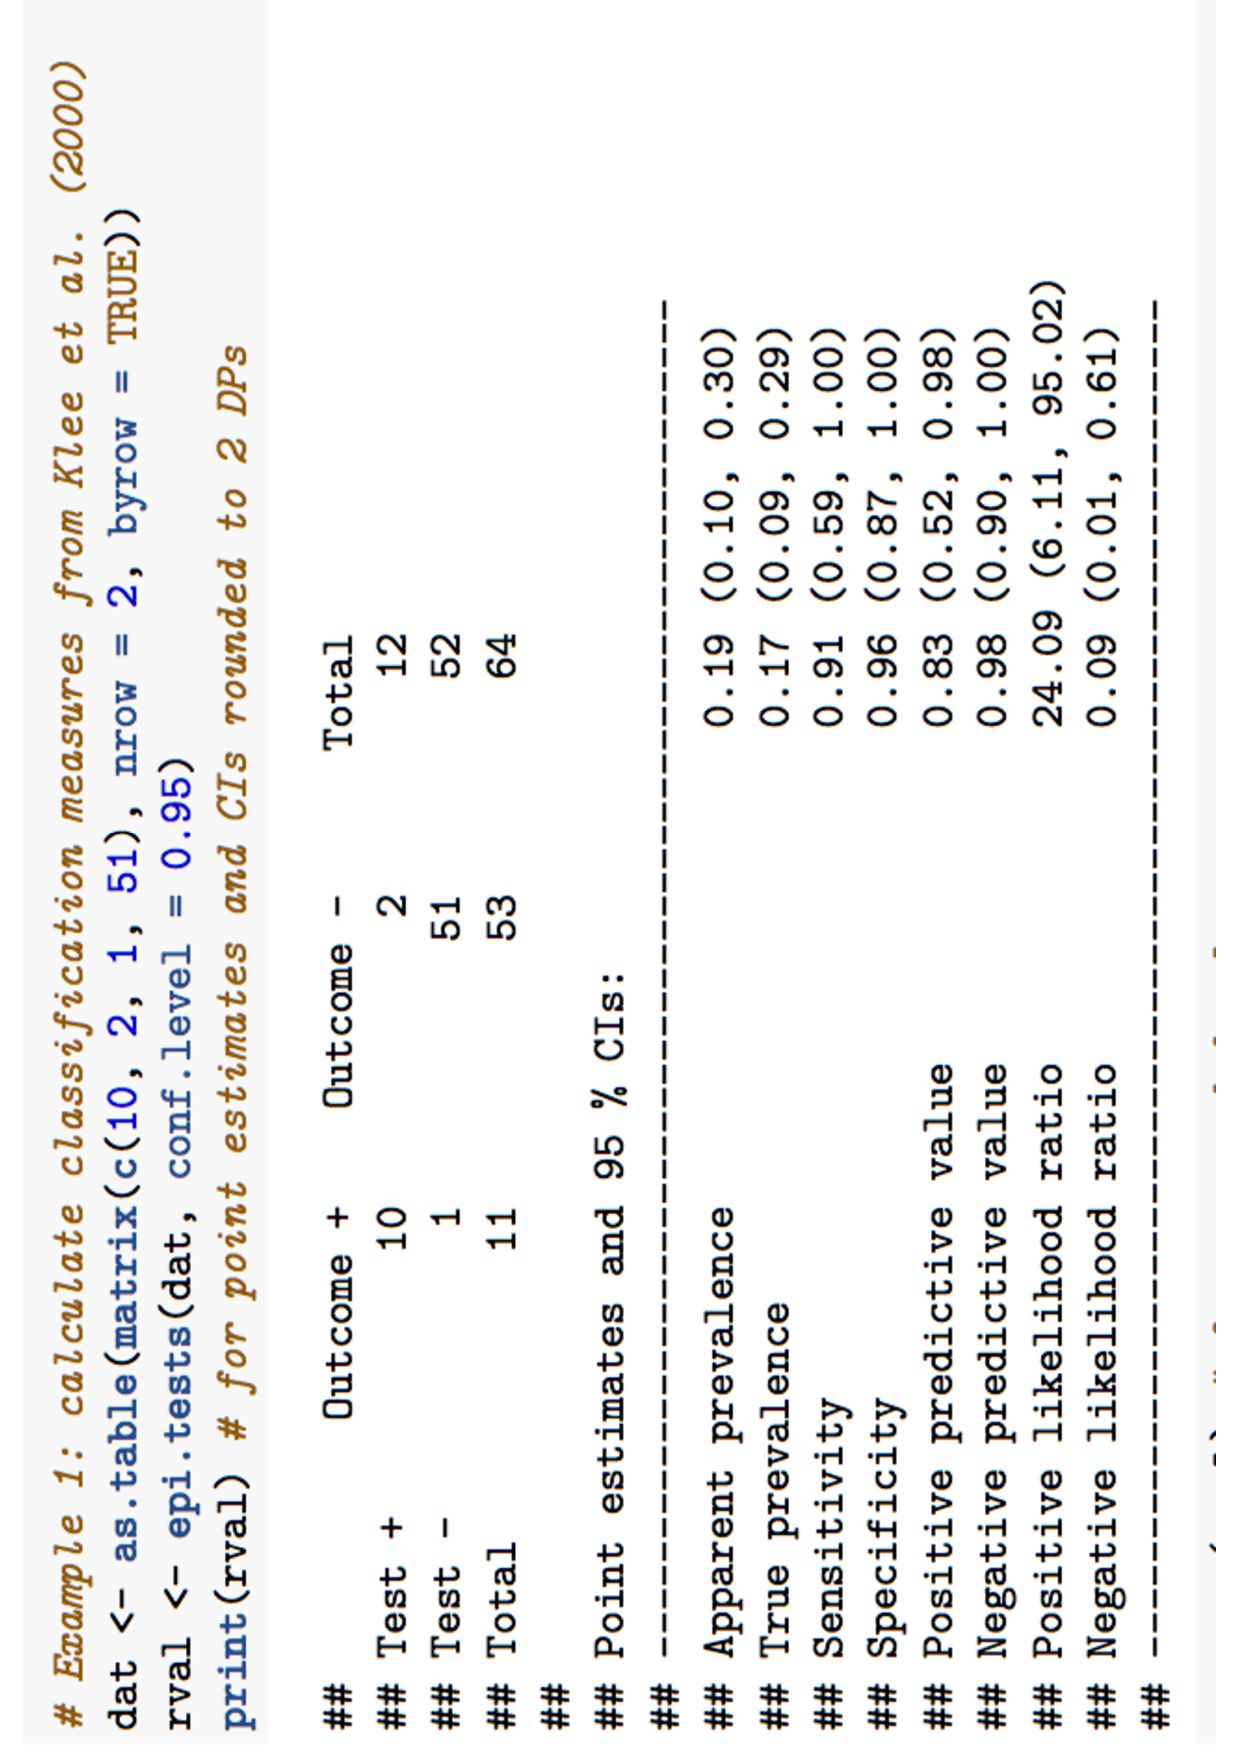
\includegraphics[angle=270, width=8cm]{images/epiR_screenshot1.pdf}
%	\end{center}	
%\end{frame}

% 26
%\begin{frame}{Post-test probabilities using R}
%	\begin{center}
%	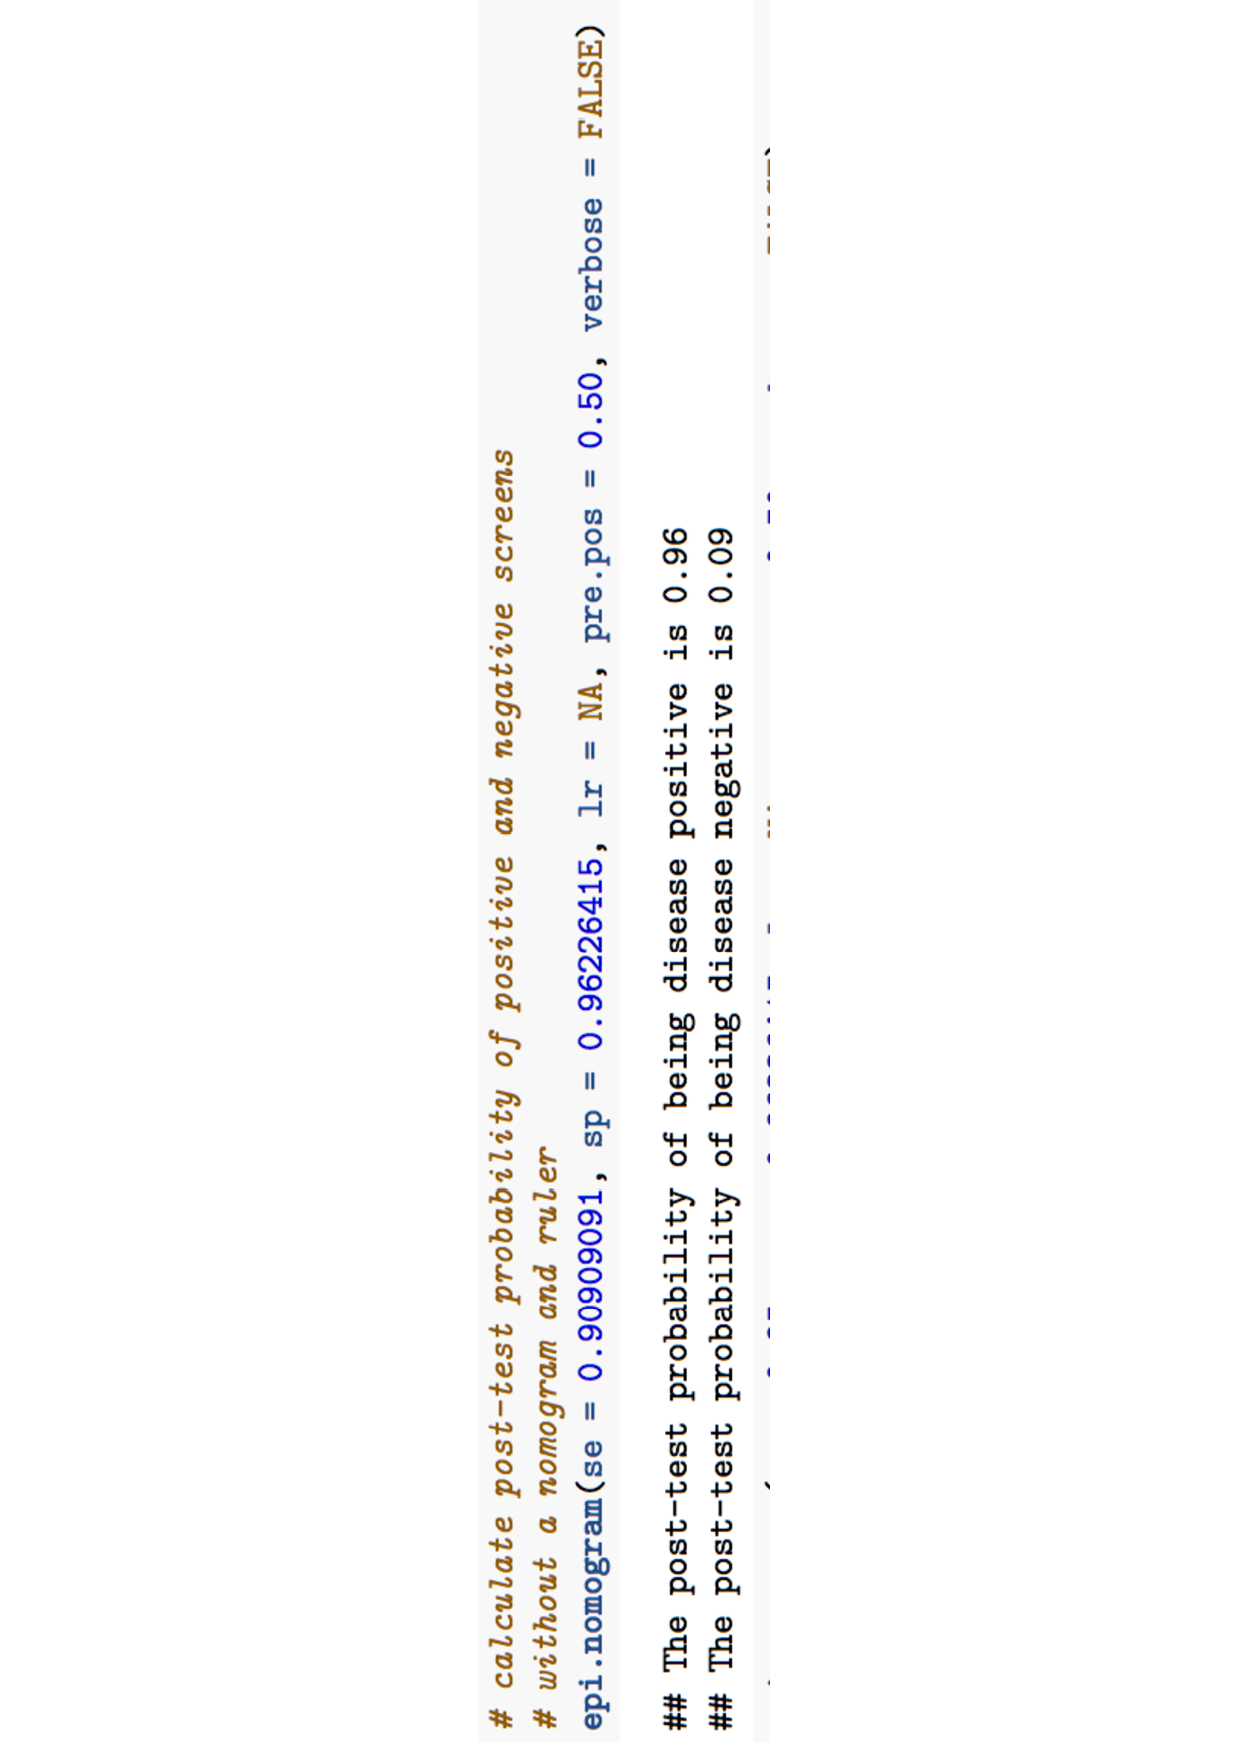
\includegraphics[angle=270, width=10cm]{images/epiR_screenshot2.pdf}
%	\end{center}
%\end{frame}

% 27
\begin{frame}{Summary of measures}
	\begin{itemize}
	\item Sensitivity and specificity tell you how accurate the test is in general. 
	\item PPV and NPV tell you what a particular test result means for a particular individual. Be cautious interpreting these, since they change with prevalence.
	\item The LR nomogram lets you calculate the probability that your client has a disorder given a particular test outcome.
	\item Be sure to take the 95\% CI into account when interpreting any of these measures.
	\end{itemize}
\end{frame}

\section{Useful Resources}

% 28
\begin{frame}{Useful resources\footnote{\tiny{All links working on 2019-03-19}}}
	\begin{block}{Diagnostic accuracy calculators}
	\footnotesize{
	\url{https://www.medcalc.org/calc/diagnostic_test.php}
	\url{https://ebm-tools.knowledgetranslation.net/calculator/diagnostic/}
	}
	\end{block}
	
	\begin{block}{Reporting standards for authors (STARD 2015)}
	\footnotesize{
	\url{http://www.equator-network.org/reporting-guidelines/stard/}
	}
	\end{block}

	\begin{block}{Reporting standards for authors of SRs and MAs of diagnostic accuracy studies (PRISMA-DTA)}
	\footnotesize{
	\url{http://jama.jamanetwork.com/article.aspx?doi=10.1001/jama.2017.19163}
	}
	\end{block}
	
	\begin{block}{Critical appraisal checklists for readers (QUADAS-2)}
\footnotesize{
	\url{http://www.bristol.ac.uk/social-community-medicine/projects/quadas/} or 
	\url{http://www.sign.ac.uk/checklists-and-notes.html}
	}
	\end{block}
\end{frame}

\section{Group Discussion}

% 29
\begin{frame}{Group discussion}
	\begin{itemize}
	\item Break up into your assigned groups.
	\item Use CADE \citep[p. 155]{Dollaghan2007a} to critically appraise the research article.
	\item Document \emph{where} you found information in the research article addressing each point.
	\end{itemize}
\end{frame}

\begin{frame}[allowframebreaks]%[shrink=15] % to reduce font size of references
	\begin{center}
	\frametitle{References}
	\bibliographystyle{apacite}
	\small\bibliography{/Users/thomasklee/Documents/Bibtex/library}
	\end{center}
\end{frame}

\end{document}